% =====================================================================
%  AetherGrid AI - UML Communication (Collaboration) Diagram, complete project
%  Single page, A3 landscape.  Compile: pdflatex aethergrid_collaboration_diagram.tex
% =====================================================================
\documentclass[10pt,a3paper]{article}
\usepackage[T1]{fontenc}
\usepackage[utf8]{inputenc}
\usepackage{helvet}
\renewcommand{\familydefault}{\sfdefault}
\usepackage[landscape,margin=0.8cm]{geometry}
\usepackage{xcolor}
\usepackage{adjustbox}
\usepackage{amssymb}
\usepackage{tikz}
\usetikzlibrary{arrows.meta,calc}
\pagestyle{empty}
\definecolor{ink}{HTML}{1F2A44}
\definecolor{hdrC}{HTML}{DDE9DD}
\definecolor{hdrP}{HTML}{D6E2F3}
\definecolor{hdrA}{HTML}{F3D4D4}
\definecolor{bdP}{HTML}{3B5B88}
\definecolor{bdA}{HTML}{9E2A2B}
\tikzset{
 obc/.style={draw=ink,line width=0.7pt,fill=hdrC,align=center,font=\fontsize{7.6}{8.6}\selectfont,text=ink,inner sep=2pt},
 obp/.style={obc,draw=bdP,fill=hdrP,text=bdP},
 obh/.style={obc,draw=bdA,fill=hdrA,text=bdA},
 link/.style={ink!70,line width=0.7pt},
 sloop/.style={-{To[length=2mm,width=2mm]},bdP,line width=0.7pt},
}
\begin{document}
\begin{center}
{\Large\bfseries AetherGrid AI \,--\, UML Communication (Collaboration) Diagram}\\[1pt]
{\small Object interaction topology of the complete system: disruption handling, batch dispatch, fleet execution, RL repositioning and verification}
\end{center}
\vspace{-6pt}
\begin{center}
\begin{adjustbox}{max width=\linewidth,max height=\dimexpr\textheight-3.4cm\relax}
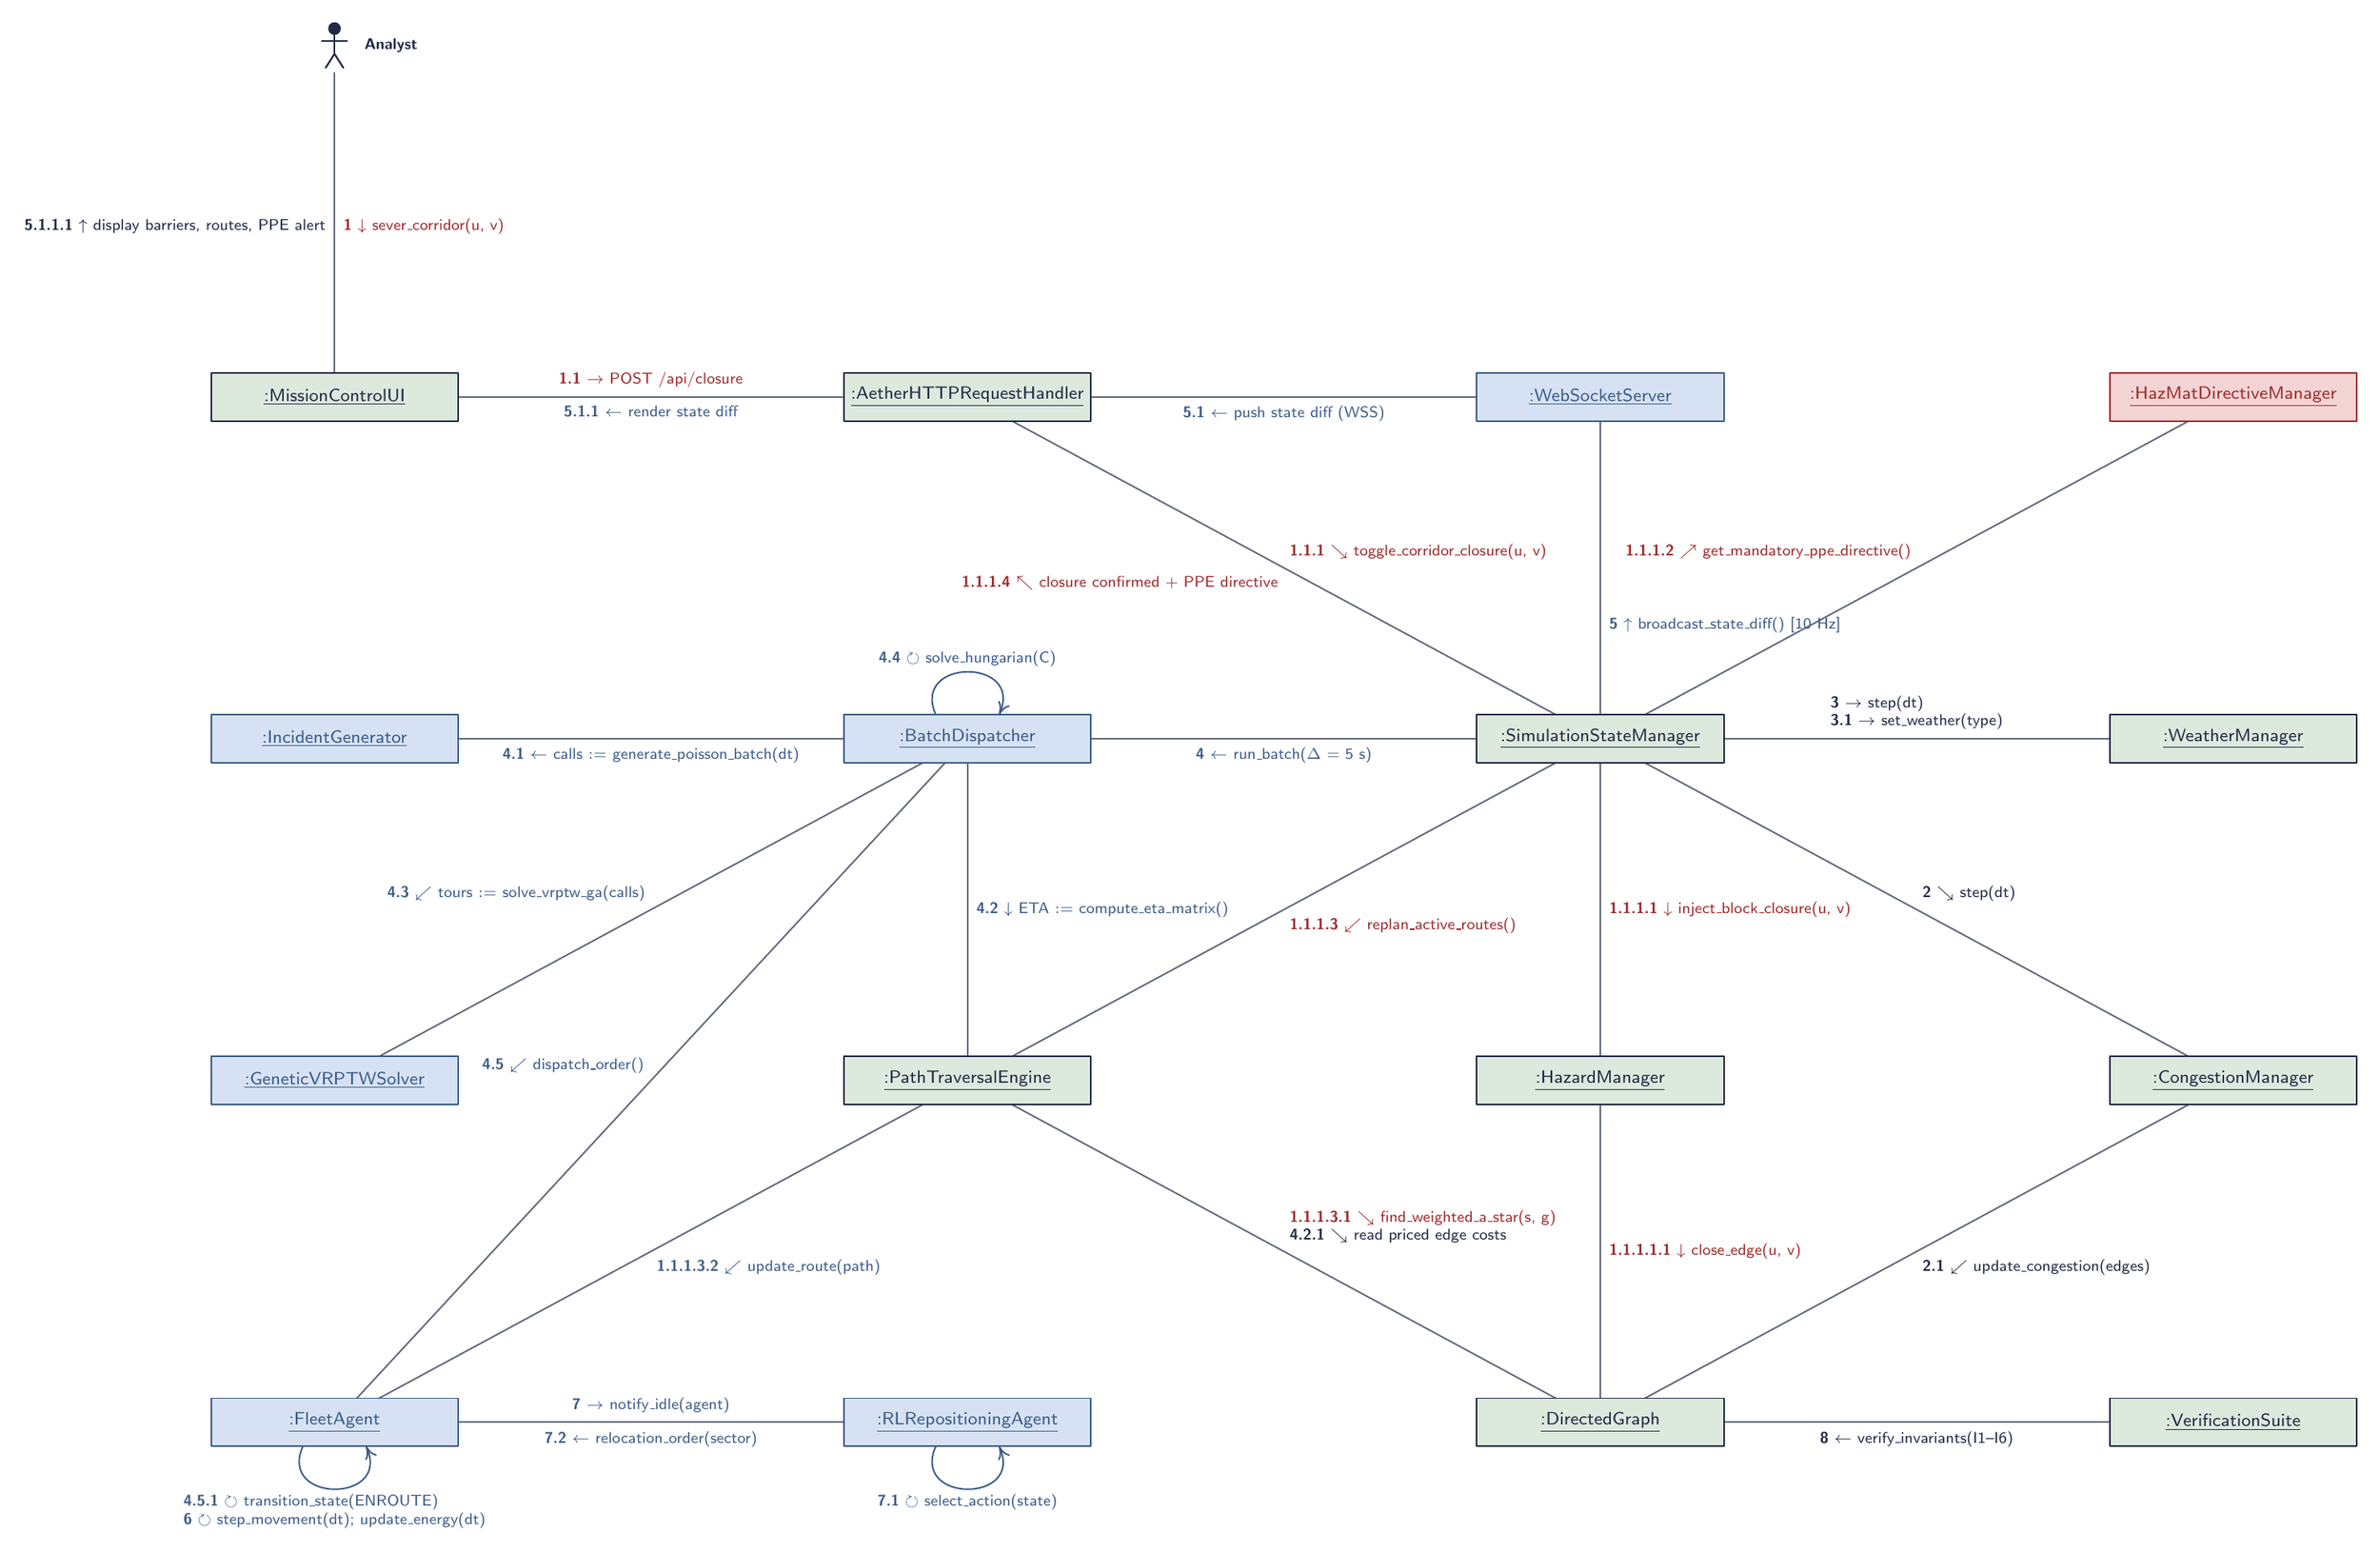
\begin{tikzpicture}[line join=round,line cap=round]
\draw[link] (0,5.12) -- (0,0);
\draw[link] (0,0) -- (10,0);
\draw[link] (10,0) -- (20,0);
\draw[link] (10,0) -- (20,-5.4);
\draw[link] (20,0) -- (20,-5.4);
\draw[link] (20,-5.4) -- (30,0);
\draw[link] (20,-5.4) -- (10,-5.4);
\draw[link] (20,-5.4) -- (30,-5.4);
\draw[link] (20,-5.4) -- (10,-10.8);
\draw[link] (20,-5.4) -- (20,-10.8);
\draw[link] (20,-5.4) -- (30,-10.8);
\draw[link] (0,-5.4) -- (10,-5.4);
\draw[link] (10,-5.4) -- (10,-10.8);
\draw[link] (10,-5.4) -- (0,-10.8);
\draw[link] (10,-5.4) -- (0,-16.2);
\draw[link] (0,-16.2) -- (10,-16.2);
\draw[link] (0,-16.2) -- (10,-10.8);
\draw[link] (10,-10.8) -- (20,-16.2);
\draw[link] (20,-10.8) -- (20,-16.2);
\draw[link] (30,-10.8) -- (20,-16.2);
\draw[link] (30,-16.2) -- (20,-16.2);
\node[anchor=west,align=left,inner sep=1pt,font=\fontsize{7.0}{8.0}\selectfont] at (0.10,2.70) {\textcolor{bdA}{\textbf{1} $\downarrow$ sever\_corridor(u, v)}};
\node[anchor=east,align=left,inner sep=1pt,font=\fontsize{7.0}{8.0}\selectfont] at (-0.10,2.70) {\textcolor{ink}{\textbf{5.1.1.1} $\uparrow$ display barriers, routes, PPE alert}};
\node[anchor=south,align=left,inner sep=1pt,font=\fontsize{7.0}{8.0}\selectfont] at (5.00,0.10) {\textcolor{bdA}{\textbf{1.1} $\rightarrow$ POST /api/closure}};
\node[anchor=north,align=left,inner sep=1pt,font=\fontsize{7.0}{8.0}\selectfont] at (5.00,-0.10) {\textcolor{bdP}{\textbf{5.1.1} $\leftarrow$ render state diff}};
\node[anchor=south west,align=left,inner sep=1pt,font=\fontsize{7.0}{8.0}\selectfont] at (15.05,-2.61) {\textcolor{bdA}{\textbf{1.1.1} $\searrow$ toggle\_corridor\_closure(u, v)}};
\node[anchor=north east,align=left,inner sep=1pt,font=\fontsize{7.0}{8.0}\selectfont] at (14.95,-2.79) {\textcolor{bdA}{\textbf{1.1.1.4} $\nwarrow$ closure confirmed + PPE directive}};
\node[anchor=north,align=left,inner sep=1pt,font=\fontsize{7.0}{8.0}\selectfont] at (15.00,-0.10) {\textcolor{bdP}{\textbf{5.1} $\leftarrow$ push state diff (WSS)}};
\node[anchor=west,align=left,inner sep=1pt,font=\fontsize{7.0}{8.0}\selectfont] at (20.10,-3.60) {\textcolor{bdP}{\textbf{5} $\uparrow$ broadcast\_state\_diff() [10 Hz]}};
\node[anchor=south east,align=left,inner sep=1pt,font=\fontsize{7.0}{8.0}\selectfont] at (24.95,-2.61) {\textcolor{bdA}{\textbf{1.1.1.2} $\nearrow$ get\_mandatory\_ppe\_directive()}};
\node[anchor=north,align=left,inner sep=1pt,font=\fontsize{7.0}{8.0}\selectfont] at (15.00,-5.50) {\textcolor{bdP}{\textbf{4} $\leftarrow$ run\_batch($\Delta$ = 5 s)}};
\node[anchor=south,align=left,inner sep=1pt,font=\fontsize{7.0}{8.0}\selectfont] at (25.00,-5.30) {\textcolor{ink}{\textbf{3} $\rightarrow$ step(dt)}\\\textcolor{ink}{\textbf{3.1} $\rightarrow$ set\_weather(type)}};
\node[anchor=south west,align=left,inner sep=1pt,font=\fontsize{7.0}{8.0}\selectfont] at (25.05,-8.01) {\textcolor{ink}{\textbf{2} $\searrow$ step(dt)}};
\node[anchor=west,align=left,inner sep=1pt,font=\fontsize{7.0}{8.0}\selectfont] at (20.10,-8.10) {\textcolor{bdA}{\textbf{1.1.1.1} $\downarrow$ inject\_block\_closure(u, v)}};
\node[anchor=north west,align=left,inner sep=1pt,font=\fontsize{7.0}{8.0}\selectfont] at (15.05,-8.19) {\textcolor{bdA}{\textbf{1.1.1.3} $\swarrow$ replan\_active\_routes()}};
\node[anchor=north,align=left,inner sep=1pt,font=\fontsize{7.0}{8.0}\selectfont] at (5.00,-5.50) {\textcolor{bdP}{\textbf{4.1} $\leftarrow$ calls $:=$ generate\_poisson\_batch(dt)}};
\node[anchor=west,align=left,inner sep=1pt,font=\fontsize{7.0}{8.0}\selectfont] at (10.10,-8.10) {\textcolor{bdP}{\textbf{4.2} $\downarrow$ ETA $:=$ compute\_eta\_matrix()}};
\node[anchor=south east,align=left,inner sep=1pt,font=\fontsize{7.0}{8.0}\selectfont] at (4.95,-8.01) {\textcolor{bdP}{\textbf{4.3} $\swarrow$ tours $:=$ solve\_vrptw\_ga(calls)}};
\node[anchor=south east,align=left,inner sep=1pt,font=\fontsize{7.0}{8.0}\selectfont] at (4.93,-10.73) {\textcolor{bdP}{\textbf{4.5} $\swarrow$ dispatch\_order()}};
\node[anchor=south,align=left,inner sep=1pt,font=\fontsize{7.0}{8.0}\selectfont] at (5.00,-16.10) {\textcolor{bdP}{\textbf{7} $\rightarrow$ notify\_idle(agent)}};
\node[anchor=north,align=left,inner sep=1pt,font=\fontsize{7.0}{8.0}\selectfont] at (5.00,-16.30) {\textcolor{bdP}{\textbf{7.2} $\leftarrow$ relocation\_order(sector)}};
\node[anchor=north west,align=left,inner sep=1pt,font=\fontsize{7.0}{8.0}\selectfont] at (5.05,-13.59) {\textcolor{bdP}{\textbf{1.1.1.3.2} $\swarrow$ update\_route(path)}};
\node[anchor=south west,align=left,inner sep=1pt,font=\fontsize{7.0}{8.0}\selectfont] at (15.05,-13.41) {\textcolor{bdA}{\textbf{1.1.1.3.1} $\searrow$ find\_weighted\_a\_star(s, g)}\\\textcolor{ink}{\textbf{4.2.1} $\searrow$ read priced edge costs}};
\node[anchor=west,align=left,inner sep=1pt,font=\fontsize{7.0}{8.0}\selectfont] at (20.10,-13.50) {\textcolor{bdA}{\textbf{1.1.1.1.1} $\downarrow$ close\_edge(u, v)}};
\node[anchor=north west,align=left,inner sep=1pt,font=\fontsize{7.0}{8.0}\selectfont] at (25.05,-13.59) {\textcolor{ink}{\textbf{2.1} $\swarrow$ update\_congestion(edges)}};
\node[anchor=north,align=left,inner sep=1pt,font=\fontsize{7.0}{8.0}\selectfont] at (25.00,-16.30) {\textcolor{ink}{\textbf{8} $\leftarrow$ verify\_invariants(I1--I6)}};
\begin{scope}[shift={(0,5.4)},line width=0.8pt,draw=ink]\fill[ink] (0,0.42) circle (0.1);\draw (0,0.32)--(0,0.02);\draw (-0.2,0.22)--(0.2,0.22);\draw (0,0.02)--(-0.14,-0.2);\draw (0,0.02)--(0.14,-0.2);\end{scope}
\node[font=\fontsize{7.4}{8.4}\selectfont\bfseries,text=ink,anchor=west] at (0.35,5.550000000000001) {Analyst};
\node[obc,minimum width=3.9cm,minimum height=0.76cm] (nUI) at (0,0) {\underline{:MissionControlUI}};
\node[obc,minimum width=3.9cm,minimum height=0.76cm] (nSV) at (10,0) {\underline{:AetherHTTPRequestHandler}};
\node[obp,minimum width=3.9cm,minimum height=0.76cm] (nWS) at (20,0) {\underline{:WebSocketServer}};
\node[obh,minimum width=3.9cm,minimum height=0.76cm] (nHZ) at (30,0) {\underline{:HazMatDirectiveManager}};
\node[obp,minimum width=3.9cm,minimum height=0.76cm] (nIG) at (0,-5.4) {\underline{:IncidentGenerator}};
\node[obp,minimum width=3.9cm,minimum height=0.76cm] (nBD) at (10,-5.4) {\underline{:BatchDispatcher}};
\node[obc,minimum width=3.9cm,minimum height=0.76cm] (nSM) at (20,-5.4) {\underline{:SimulationStateManager}};
\node[obc,minimum width=3.9cm,minimum height=0.76cm] (nWM) at (30,-5.4) {\underline{:WeatherManager}};
\node[obp,minimum width=3.9cm,minimum height=0.76cm] (nGA) at (0,-10.8) {\underline{:GeneticVRPTWSolver}};
\node[obc,minimum width=3.9cm,minimum height=0.76cm] (nPE) at (10,-10.8) {\underline{:PathTraversalEngine}};
\node[obc,minimum width=3.9cm,minimum height=0.76cm] (nHM) at (20,-10.8) {\underline{:HazardManager}};
\node[obc,minimum width=3.9cm,minimum height=0.76cm] (nCM) at (30,-10.8) {\underline{:CongestionManager}};
\node[obp,minimum width=3.9cm,minimum height=0.76cm] (nFA) at (0,-16.2) {\underline{:FleetAgent}};
\node[obp,minimum width=3.9cm,minimum height=0.76cm] (nRL) at (10,-16.2) {\underline{:RLRepositioningAgent}};
\node[obc,minimum width=3.9cm,minimum height=0.76cm] (nDG) at (20,-16.2) {\underline{:DirectedGraph}};
\node[obc,minimum width=3.9cm,minimum height=0.76cm] (nVR) at (30,-16.2) {\underline{:VerificationSuite}};
\draw[sloop] (9.5,-5.0200000000000005) .. controls (9.1,-4.12) and (10.9,-4.12) .. (10.5,-5.0200000000000005);
\node[anchor=south,align=left,inner sep=1pt,font=\fontsize{7.0}{8.0}\selectfont] at (10.00,-4.30) {\textcolor{bdP}{\textbf{4.4} $\circlearrowright$ solve\_hungarian(C)}};
\draw[sloop] (-0.5,-16.58) .. controls (-0.9,-17.479999999999997) and (0.9,-17.479999999999997) .. (0.5,-16.58);
\node[anchor=north,align=left,inner sep=1pt,font=\fontsize{7.0}{8.0}\selectfont] at (0.00,-17.30) {\textcolor{bdP}{\textbf{4.5.1} $\circlearrowright$ transition\_state(ENROUTE)}\\\textcolor{bdP}{\textbf{6} $\circlearrowright$ step\_movement(dt); update\_energy(dt)}};
\draw[sloop] (9.5,-16.58) .. controls (9.1,-17.479999999999997) and (10.9,-17.479999999999997) .. (10.5,-16.58);
\node[anchor=north,align=left,inner sep=1pt,font=\fontsize{7.0}{8.0}\selectfont] at (10.00,-17.30) {\textcolor{bdP}{\textbf{7.1} $\circlearrowright$ select\_action(state)}};
\end{tikzpicture}
\end{adjustbox}
\end{center}
\vspace{2pt}
\begin{center}

\begin{tikzpicture}[font=\footnotesize]
 \node[obc,minimum width=1.3cm,minimum height=0.5cm] at (0,0) {}; \node[anchor=west,text=ink] at (0.8,0) {Implemented object};
 \node[obp,minimum width=1.3cm,minimum height=0.5cm] at (6,0) {}; \node[anchor=west,text=ink] at (6.8,0) {Planned object};
 \node[obh,minimum width=1.3cm,minimum height=0.5cm] at (11.6,0) {}; \node[anchor=west,text=ink] at (12.4,0) {HazMat safety object};
 \draw[link] (16.8,0)--(18.2,0); \node[anchor=west,text=ink] at (18.4,0) {Link};
 \node[anchor=west,text=ink] at (20.2,0) {Messages: number, arrow $\rightarrow\nearrow\uparrow$ gives direction, nesting 1 / 1.1 / 1.1.1 gives call order;};
 \node[anchor=west,text=bdA] at (20.2,-0.55) {red = disruption / HazMat};
 \node[anchor=west,text=bdP] at (26.0,-0.55) {blue = planned subsystem};
 \node[anchor=west,text=ink] at (31.8,-0.55) {$\circlearrowright$ = self message};
\end{tikzpicture}
\end{center}
\end{document}
